\section {Aproximação da Equação de Helmholtz}

Para cada ponto $u$ do domínio, desejamos calcular $R(u) = A(u)e^{i\phi(u)}$. Consideremos, então, o sinal de um ponto fixo. Ao entrar em equilíbrio, o sinal $s(t)$ desse ponto poderá ser representado por $s(t) = A \cos(\omega t + \phi)$. Se calcularmos o valor médio\footnote{O valor médio $\mean{f}$ de uma função $f(t)$ é definido por $$\mean{f} = \frac{\int_a^b f(t)}{b-a}$$} $\mean{s}$ do valor absoluto sinal ao longo de um certo período, obteremos $\mean{|s|} = \frac{2A}{\pi}$. Logo, se soubermos $\mean{|s|}$ e $s(t)$ para um certo $t$, podemos calcular $A$ e $\phi$: 

\begin{equation}
	\begin{cases}
		A = \frac{\pi\mean{|s|}}{2}\\
		\phi = \arccos \left(\frac{s(t)}{A}\right) - \omega t
	\end{cases}
	\label{eq:amplitude_phase_estimation}
\end{equation}

Na nossa implementação, o valor médio do sinal de cada elemento do domínio é calculado utilizando uma \emph{Weighted Moving Average} (WMA), isto é:

\begin{equation}
	\mean{s}_{t} = \alpha\mean{s}_{t-1} + (1-\alpha)s(t)
\end{equation}

A amplitude $A$ e a fase $\phi$ são calculados a cada timestep utizando a fórmula \eqref{eq:amplitude_phase_estimation}. O valor médio de $A$ e $\phi$ também são calculados utilizando uma WMA. Em todos os casos, utilizamos $\alpha = 0.95$.

\begin{figure}[ht]
\centering
\begin{subfigure}{0.5\textwidth}
	\centering
	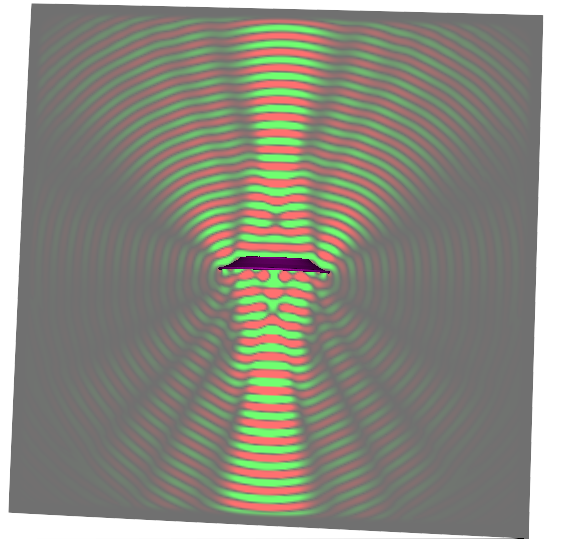
\includegraphics[width=\textwidth]{algorithm/plate_mode_a.png}
	\caption{Computado}\label{fig:wave_plates_a}
\end{subfigure}%
\begin{subfigure}{0.5\textwidth}
	\centering
	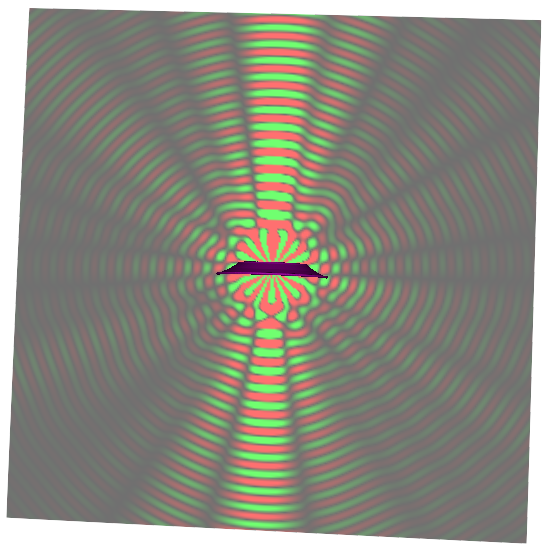
\includegraphics[width=\textwidth]{algorithm/plate_mode_b.png}
	\caption{Estimado com multipolos com $\bar{n}$ = 16}
	\label{fig:wave_plates_b}
\end{subfigure}
\caption[Equação da onda nos pratos]{Equação da onda nos pratos}
\label{fig:wave_plates}
\end{figure}